\documentclass[crop,border={2pt 2pt 2pt 2pt},tikz]{standalone}
\usepackage{braket}
\usepackage{bbold}
\usepackage{bm}
\usepackage{amsmath}
\usepackage{tikz-3dplot}
% \usepackage{physics}

\usetikzlibrary{backgrounds,decorations.markings, calc}
\tikzset{>=latex}
\tikzset{->-/.style={decoration={
  markings,
  mark=at position .55 with {\arrow{>}}},postaction={decorate}}}
\begin{document}
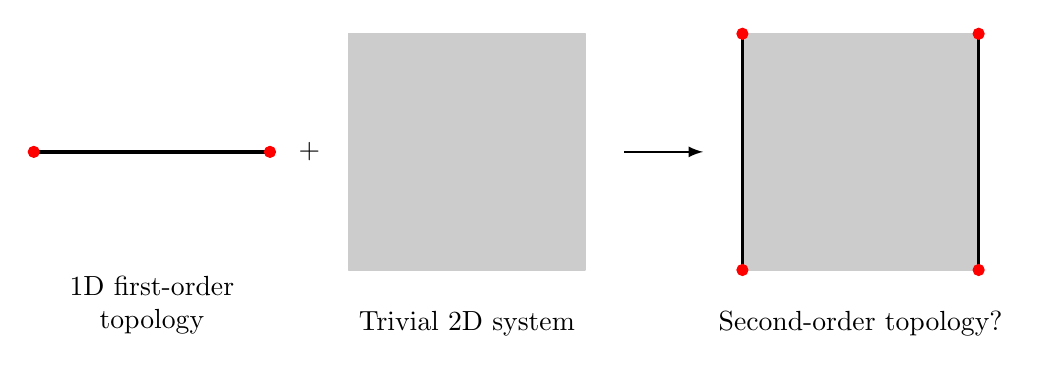
\begin{tikzpicture}[line join = round]
    \draw[very thick] (0,0) -- (3,0);
    \draw[fill, red] (0,0) circle (2pt) (3,0) circle (2pt);
    \node[] at (3.5,0) {$+$};
    \draw[fill, black!20!white] (4, -1.5) rectangle (7, 1.5);
    \draw[->, thick] (7.5,0) -- (8.5,0);
    \draw[fill, black!20!white] (9, -1.5) rectangle (12, 1.5); 
    \draw[very thick] (9,-1.5) -- (9,1.5);
    \draw[fill, red] (9,-1.5) circle (2pt) (9,1.5) circle (2pt);
    \draw[very thick] (12,-1.5) -- (12,1.5);
    \draw[fill, red] (12,-1.5) circle (2pt) (12,1.5) circle (2pt);
    \node[anchor=north, align=center] at (1.5, -1.45) {$1$D first-order \\ topology};
    \node[anchor=north, align=center] at (5.5, -1.9) {Trivial $2$D system};
    \node[anchor=north, align=center] at (10.5, -1.9) {Second-order topology?};


\end{tikzpicture}
\end{document}